\mainmatter

\chapter{Einleitung}\label{chap:introduction}
%% 1. Hintergrund und Kontext
%  Einführung in das Thema: Eine kurze Darstellung des übergeordneten Themas der Arbeit, um dem Leser ein allgemeines Verständnis zu geben.
%  Relevanz und Bedeutung: Erklärung, warum das Thema wichtig ist, und seine Relevanz im akademischen, industriellen oder gesellschaftlichen Kontext.
% 2. Problemstellung
%  Beschreibung des Problems: Detaillierte Darstellung des spezifischen Problems oder der Fragestellung, die in der Arbeit behandelt wird.
%  Konkrete Herausforderungen: Aufzeigen der spezifischen Herausforderungen und Fragen, die sich aus dem Problem ergeben.
% 3. Zielsetzung und Forschungsfragen
%  Ziele der Arbeit: Klar formulierte Ziele, die mit der Arbeit erreicht werden sollen.
%  Forschungsfragen: Präzise Forschungsfragen, die die Arbeit zu beantworten versucht.
% 4. Methodik
%  Überblick über die Methoden: Kurze Beschreibung der methodischen Ansätze, die verwendet werden, um die Forschungsfragen zu beantworten.
%  Datenquellen und Analysen: Hinweise auf die verwendeten Datenquellen und die Art der Analysen.
% 5. Aufbau der Arbeit
%  Kapitelübersicht: Kurzbeschreibung der Struktur der Arbeit, um dem Leser einen Überblick zu geben, wie die Arbeit organisiert ist.
%  Kapitelinhalte: Kurze Zusammenfassungen dessen, was in den einzelnen Kapiteln behandelt wird.
% 6. Abgrenzungen
%  Eingrenzung des Themas: Festlegung der Grenzen der Untersuchung, um den Umfang der Arbeit klarzustellen.
%  Einschränkungen und Annahmen: Diskussion über die Einschränkungen der Arbeit und die Annahmen, die gemacht wurden.

%\section{Hintergrund und Kontext}
Durch die zunehmende Globalisierung und Digitalisierung wird die Gesellschaft der Gegenwart und Zukunft geprägt. Der Ausbau von Hochgeschwindigkeitsnetze und die globale Corona-Pandemie haben diese Entwicklung noch einmal beschleunigt. Immer mehr Unternehmen erkennen die Potenziale der Digitalisierung und stellen ihre Geschäftsprozesse um. Ganze Wertschöpfungsketten werden auf cloudbasierte Umgebungen umgestellt. Angefangen bei der Kommunikation, über Beschaffung und Produktion bis zum Verkauf der Waren und Dienstleistungen, vergleiche mit \parencite[Seite 21 ff.]{banholzer-2020} und \cite{oswald-2022}. In allen Stufen der Prozesse kommen webbasierte Anwendungen zum Einsatz, um die Kommunikation der Anwender mit den Systemen zu ermöglichen oder Schnittstellen für die Datenübertragung zwischen den verschiedenen Systemen zu gewährleisten. Durch wachsende Anzahl von Web-Anwendungen wächst auch der Druck für die Entwicklungsfirmen, ihre Anwendungen den schnell und oft wechselnden Kundenanforderungen anzupassen.\vspace{0.2cm}

Durch diesen Prozess getrieben, müssen Entwicklungsfirmen in immer kürzeren Release-Zyklen Softwarekomponenten hinzufügen und vorhandene erweitern. Gleichzeitig wachsen aber auch die Anforderungen an Stabilität und Sicherheit der cloudbasierten Anwendungen, sowie der Bedarf an kostengünstigeren IT-Abläufen (Beweis fehlt). Ein weiteres Problem ist der wachsende Fachkräftemangel in der Wirtschaft und die damit verbundenen steigenden Gehälter der Entwickler (Beweis fehlt).\vspace{0.2cm}

Die Verwendung künstlicher Intelligenz bei der Programmierung gewinnt immer mehr an Bedeutung. Eine Technologie die im besonderen Maße an dieser Entwicklung beteiligt ist, sind die Large Language Models. Insbesondere mit der Veröffentlichung vom ChatGPT wurde hier ein regelrechter Hype um die \acrshort{LLM}s ausgelöst. Diese Modelle erlauben eine Softwareentwicklung mit natürlicher Sprache. Tiefe Kenntnisse der verwendeten Programmiersprache sind nicht mehr in dem Maße erforderlich, wie ohne LLMs.\vspace{0.2cm}


\section{Problemstellung}
So groß der Hype um Künstliche Intelligenz auch sein mag, zurzeit kann KI nicht alle Anforderungen selbstständig lösen. Dies sollte auch bei der Verwendung von KI generierten Inhalten und Programmcodes beachtet werden.

\epigraph[
	source={Vattenfall Online},
	etc={ KI für Unternehmen – die Grenzen der KI},
	author and source indent=0.5cm,
	dash=,
	after skip=0.5cm
]{KI denkt nicht, KI trifft keine Entscheidungen. Eine KI antwortet auf eine Eingabe nicht mit der besten Antwort, sondern mit der Wahrscheinlichsten.}

Der Mensch muss die generierten Ergebnisse überprüfen, ehe erstellte Programmcodestücke in vorhandene Programme eingefügt und in Produktionsumgebungen implementiert werden.\vspace{0.3cm}

Viele Entwickler setzen auf Chatbots, wie ChatGPT oder Gemini zur Generierung von Code, wie eine Umfrage von \textit{stackoverflow} vom Mai 2024 zeigt \cite{noauthor_developers_2024}. Gleichzeitig wachsen auch die technischen Schulden bei Softwareprojekten, da diese Modelle nicht für die Entwicklung von Software optimiert sind (Beweis fehlt).\vspace{0.2cm}

%\subsection{Herausforderungen bei der Entwicklung von Webanwendungen}

%\subsection{Potenzial von LLMs in der Webentwicklung}


\section{Zielsetzung und Forschungsfragen}
Diese Arbeit soll eine Auswahl von Modellen evaluieren und dessen Brauchbarkeit für die Softwareentwicklung aufzeigen. Die Modellauswahl wird von der Seite \href{https://evalplus.github.io/leaderboard.html}{EvalPlus Leaderboard} abgeleitet. Hier werden Modelle gewählt, welche erstere Plätze belegen, aber zum Vergleich auch Modelle aus dem Mittelfeld.\vspace{0.2cm}

Des Weiteren soll gezeigt werden, ob die automatisierte Verwendung beider Techniken eine Effizienz und Effektivität des Entwicklungsprozesses gesteigert werden kann.


\section{Aufbau der Arbeit}
Ein paar Worte zum Aufbau dieser Arbeit. Im Kapitel \ref{chap:state_of_research} wird der aktuelle Stand der Forschung vorgestellt und Erkenntnisse anderer Arbeiten diskutiert. Die in dieser Arbeit verwendetet Methoden, werden im Kapitel \ref{chap:methodology} behandelt. Die Implementierung der Test LLMs wird in Kapitel \ref{chap:implementation} besprochen und in Kapitel \ref{chap:evaluation} die Ergebnisse evaluiert. Bevor in Kapitel \ref{chap:conclusion} auf mögliche Folgearbeiten eingegangen wird, gibt es in Kapitel \ref{chap:application_scenarios} Anwendungsszenarien, die zu den Ergebnissen dieser Arbeit geführt haben.


\section{Abgrenzung}
Ausschluss anderer Anwendungsbereiche.

Rechtliche und ethische Überlegungen werden nur am Rande berücksichtigt.

\chapter{Grundlagen}\label{chap:basics}
%In diesem Kapitel werden Grundlagen besprochen die eine Relevanz für diese Arbeit haben. Die angesprochenen Bereiche können nur oberflächlich einen kleinen Einstieg in die jeweiligen Teilgebiete geben.\vspace{0.2cm}

Die Forschungsbereiche der großen Sprachmodelle, kurz \acrshort{LLM} [eng. Large Language Model], ist ein Teilgebiet von Deep Learning und der Forschung von der Verarbeitung natürlicher Sprache, kurz \acrshort{NLP} [eng. Natural Language Processing]. Die Grafik \ref{img:classification_of_terms} zeigt die Einordnung der Bereiche.

\begin{figure}[!ht]
	\includegraphics[width=0.8\textwidth]{content/chapter_basics/images/einordnung_bezeichnungen.eps}
	\centering
	\caption{LLMs im Kontext der Forschungsbereiche von KI}
	\label{img:classification_of_terms}
\end{figure}


\section{Künstliche Intelligenz}
Die künstliche Intelligenz hat bereits in viele Unternehmensprozesse Einzug gehalten. Besonders die generative KI, mit ihren großen Sprachmodellen wird in den nächsten Jahren immer weiter in die Unternehmensbereiche vorstoßen und viele Aufgaben übernehmen. Entscheider und Führungspersonal versprechen sich von der Technologie nicht nur effizientere Prozesse, sondern auch Kosteneinsparungen.\vspace{0.2cm}

Eine explizite Definition für \textit{künstliche Intelligenz} ist zurzeit noch nicht einheitlich erfolgt. Geschuldet ist diese Tatsache, dass der Begriff \textit{Intelligenz} nicht eindeutig definiert ist. Somit finden sich viele Versuche eine Definition für künstliche Intelligenz herzuleiten. In dieser Arbeit wird als Definition für die Künstliche Intelligenz, die aus \cite[6 ff.]{definition_ki2019} verwendet.

\epigraph[
	author={Bitkom e.V.},
	text indent=0.5cm,
	after skip=-1.0cm
	]{
	Systeme der künstlichen Intelligenz (KI-Systeme) sind vom Menschen entwickelte Softwaresysteme (und gegebenenfalls auch Hardwaresysteme), die in Bezug auf ein komplexes Ziel auf physischer oder digitaler Ebene handeln, indem sie ihre Umgebung durch Datenerfassung wahrnehmen, die gesammelten strukturierten oder unstrukturierten Daten interpretieren, Schlussfolgerungen daraus ziehen oder die aus diesen Daten abgeleiteten Informationen verarbeiten, und über das bestmögliche Handeln zur Erreichung des vorgegebenen Ziels entscheiden. KI-Systeme können entweder symbolische Regeln verwenden oder ein numerisches Modell erlernen, und sind auch in der Lage, die Auswirkungen ihrer früheren Handlungen auf die Umgebung zu analysieren und ihr Verhalten entsprechend anzupassen.
}

%(\href{https://www.bitkom.org/sites/main/files/file/import/171012-KI-Gipfelpapier-online.pdf}{Wirtschaftliche Bedeutung ...}, 26 ff.).

%Die folgenden Kapitel werden auf die Teilbereiche der künstlichen Intelligenz eingehen, welche für die Entwicklung der großen Sprachmodelle essenziell sind.
Aus dem Forschungsgebiet der künstlichen Intelligenz ist für die großen Sprachmodelle der Bereich des \glqq Deep Learning\grqq \ besonders interessant. Hier findet die Überschneidung mit dem Bereich der NLP statt, welche massiv dazu betrug, dass die großen Sprachmodelle diesen Erfolg erfahren.

\subsection{Maschinelles Lernen}
Als Teilgebiet der künstlichen Intelligenz befasst es sich mit dem Problem wie Maschinen Lernen und Denken können. Wobei hier nicht von selbstständigem Lernen und Denken gesprochen werden kann, sondern lediglich von Imitieren dieser Prozesse. Aber \acrshort{ML} ist sehr wohl in der Lage aus großen Datenmengen komplexe Muster und Funktionen zu erkennen. Für das maschinelle Lernen gibt es mehrere Formen von Lernparadigmen.\vspace{0.2cm}

Beim \textit{überwachten Lernen} sind für die Eingaben der Trainingsdaten dazugehörige Ausgaben, die Labels definiert. Das Ziel ist es eine Funktion zu trainieren um künftige Eingaben korrekt klassifizieren oder vorhersagen zu können. Dieses Lernparadigma wird häufig eingesetzt, wenn es sich um Regressionens- und Klassifizierungsprobleme handelt.\vspace{0.2cm}

Die gelabelten Ausgaben sind beim \textit{unüberwachten Lernen} nicht vorhanden. Hierbei wird beispielsweise durch Clustering oder Dimensionsreduktion versucht Muster und Strukturen zu erkennen. Des Weiteren soll die Methode helfen Anomalien in Daten zuerkennen aber Assoziationen zwischen Datenobjekten zu finden.\vspace{0.2cm}

Das \textit{selbst überwachte Lernen} ermöglicht es Modellen, sich selbst zu überwachen ohne gelabelte Daten. Hierbei lernen die Algorithmen einen Teil der Eingaben von anderen Teilen und generieren automatisch Labels. So werden unüberwachten Problemen in überwachte Probleme überführt. Diese Art des Lernens ist u.a. besonders nützlich bei NLP, da hier die Trainingsdaten in großer Anzahl vorliegen\vspace{0.2cm}

Beim \textit{verstärkten Lernen} (engl. Reinforcement Leraning) werden die Systeme mit Belohnung un Strafe trainiert. Das System wird aufgrund seines Handelns bewertet, dadurch wird es ermutigt gute Praktiken weiterzuverfolgen und schlechte zu verwerfen. Das Lernen wird häufig bei der Videospielentwicklung und in der Robotik eingesetzt.\vspace{0.2cm}

Eine weitere Art ist das \textit{Semi-überwachte Lernen} die eine Kombination aus unüberwachten und überwachten Lernens ist. Bei diesem Lernen steuern kleine gelabelte Datensätze eine große Menge an ungelabelten Datensätzen. Die verwendeten Technologien von GANs (Generative Adversarial Networks) bis zu Diffusionsmodellen sind in der Lage neue Inhalte zu schaffen und sind Voraussetzungen für heutige generative KI.\vspace{0.2cm}


\subsection{Neuronale Netze}
Neuronale Netze oder auch künstliche neuronale Netze (\acrshort{KNN}) sind spezifische Typen des maschinellen Lernens. Sie sollen die biologischen Neuronen des Gehirns nachempfinden. Die Abbildung \ref{img:biological_neuron} von \cite{pahl-2024} zeigt eine stark vereinfachte biologische Nervenzelle.

\begin{figure}[!ht]
	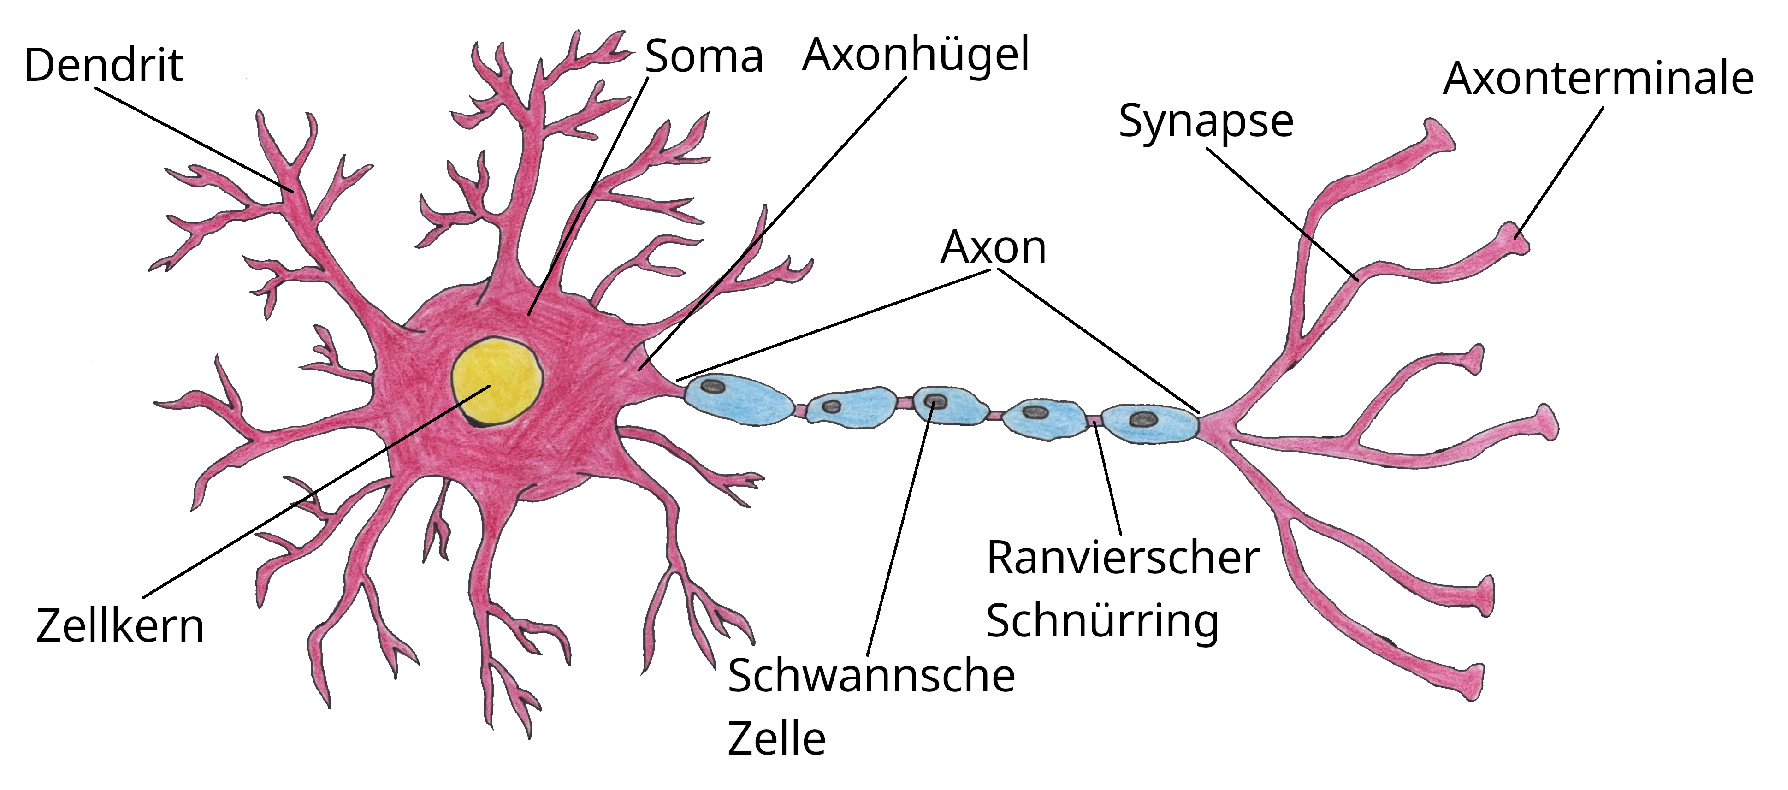
\includegraphics[width=0.8\textwidth]{content/chapter_basics/images/biological_neuron.eps}
	\centering
	\caption{Biologische Nervenzelle}
	\label{img:biological_neuron}
\end{figure}

Bei Nervenzellen werden elektrische Eingangssignale über Dendriten aufgenommen und in den Zellkern geleitet. Dort werden die eingehenden Signale zusammen geführt und es bildet sich das Aktionspotential. Übersteigt es das Schwellenpotential der Zelle, so wird das Signal über das Axon abgeleitet, die Nervenzelle \glqq \textit{feuert}\grqq.\vspace{0.2cm}

Die kleinste Einheit in künstlichen neuronalen Netzen sind die Neuronen. Sie sind den biologischen Nervenzellen nachempfunden.

\begin{figure}[!ht]
	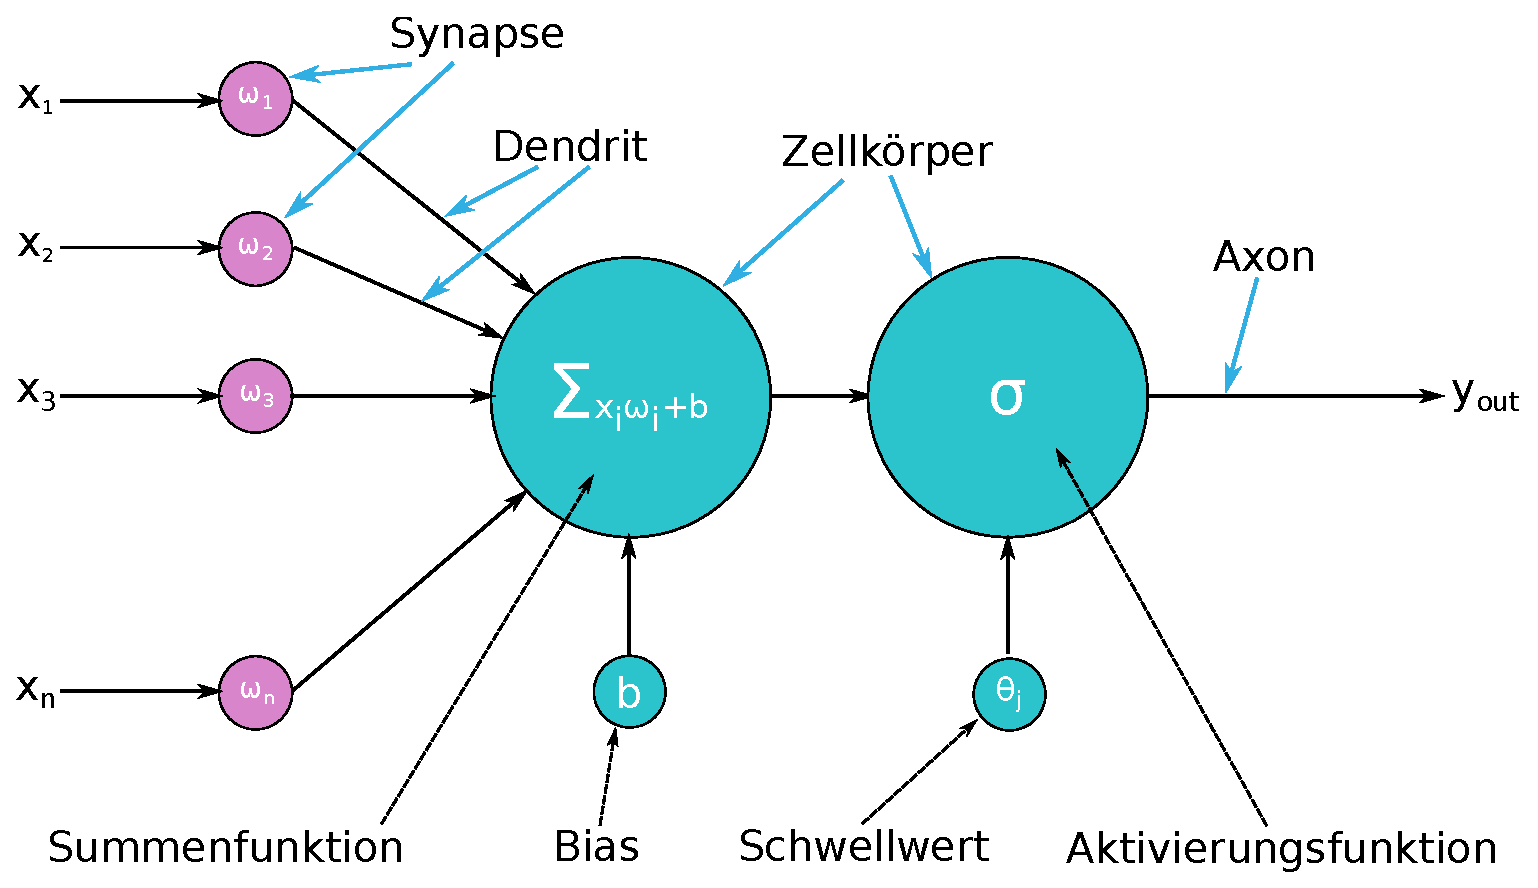
\includegraphics[width=0.8\textwidth]{content/chapter_basics/images/artificial_neuron.eps}
	\centering
	\caption{Künstliche Nervenzelle}
	\label{img:artificial_neuron}
\end{figure}

Sie haben als Eingangswert einen Vektor und als Ausgangssignal ein Skalar. Außer in der Eingabe Schicht ist jedes Eingangssignal $x_n$ ein Ausgangssignal $y_{out}$ eines anderen Neuron. Die Wichtungen der Eingangssignale modellieren den synaptischen Spalt zwischen zwei biologischen Nervenzellen. Dieser kann ebenfalls verstärkten oder hemmend wirken. Alle Eingangssignale zusammen mit den Wichtungen, werden durch die Summenfunktion aufaddiert. Im Anschluss wird das \gls{bias} mit eingerechnet. Die Formel \ref{eq:sum_function} zeigt die Summenfunktion für $n$ Eingangssignale mit Beachtung des Bias Wert.

\begin{equation} \label{eq:sum_function}
	y_{sum} = x_{1} + x_{2} + \dots + x_{n} + b
\end{equation}

Nach der Summenfunktion wird das Signal an die Aktivierungsfunktion übergeben. Diese Funktion leitet ein Signal erst weiter, wenn ein festgelegter Schwellwert überschritten wird. Die Analogie zur biologischen Nervenzelle ist das Aktionspotential, welches durch die Reize anderer Nervenzellen aufgebaut wird und wie beim künstlichen Neuron führt das Überschreiten eines Schwellenwertes dazu, dass das Neuron \glqq feuert\grqq. Die Formel \ref{eq:activation_function} zeigt das Verhalten einer \glqq Binary Step\grqq -Aktivierungsfunktion mit vorgegebenen Schwellenwert $S$.

\begin{equation}\label{eq:activation_function}
	\sigma (y_{sum}) = \left\{
	\begin{array}{cl}
		1: & y_{sum} > S \\
		0: & sonst \\
	\end{array}
	\right.
\end{equation}

Neben dieser einfachen Aktivierungsfunktion wie die \textit{Binary Step} gibt es viele weitere Aktivierungsfunktionen, beispielsweise die \textit{Sigmoidfunktion} oder \textit{ReLU (Rectified Linear Unit)} Funktion. Diese Aktivierungsfunktionen verwenden für die Berechnung immer das Ergebnis der Summenfunktion. Es gibt auch Aktivierungsfunktionen die alle Neuronen einer Schicht zur Berechnung verwenden. Zu diesen Funktionen zählen u.a. die Softmax- und die Maxout-Aktivierungsfunktion.\vspace{0.2cm}

Das eben beschriebene Neuronen-Modell ist ein einfaches Modell, welches oft in Netzen wie \textit{Feedforward Neural Netzwerke (FNN)}, \textit{Rekurrente neuronale Netze (RNNs)} oder \textit{Long Short-Term Memory Networks (LSTM)} Anwendung findet. Andere Neuronen-Modelle wie beispielsweise das \textit{Leaky-Integrate-And-Fire} Modell, finde seine Anwendung in gepulsten Netzwerken. Mit diesen mathematischen Modellen wird versucht das biologische Nervensystem nachzubilden, mit all seinen stärken und schwächen. Die Forschung hat in den letzten Jahren große Fortschritte gemacht, mit immer besser werdender Technik und Verständnis der biologischen ist das Potenzial der neuronalen Netze noch nicht erschöpft.


\subsection{Deep Learning}
Das Teilgebiet \textit{Deep Learning} versucht möglichst präzise Vorhersagen und Entscheidungen aus komplexen Daten zutreffen. Hierfür werden tiefe neuronale Netze verwendet. Das sind Netze mit vielen Hidden Layern zwischen der Ein- und Ausgabeschicht. Diese Strukturen erlauben die Verarbeitung und Analyse komplexer Datenmuster.


\section{Natural Language Processing}
Natural Language Processing ist ein Teilgebiet der Informatik und nutzt Deep Learning. NLP soll es digitalen Systemen in die Lage versetzen Texte und Sprachen zu erkennen, um diese zu verstehen und verarbeiten zu können. Dabei muss NLP die Bedeutung (Semantik) der Texte erkennen, die Grammatik und Beziehungen zwischen den Teilen der Sprache herstellen, Wortarten wie Verben, Adjektive und Nomen spezifizieren, sowie verschiedene Formen der Sprache beherrschen wie beispielsweise Prosa oder wissenschaftliches Schreiben.\vspace{0.2cm}

NLP wird aber auch in anderen Bereichen eingesetzt. Mithilfe von NLP können Bilder generiert, Suchmaschinen abgefragt, Chatbots für den Kundenservice betrieben werden und Sprachassistenten wie Amazon Alexa, MS Cortana und Apple Siri nutzen ebenfalls die NLP Techniken.\vspace{0.2cm}

Zunehmend findet NLP Einsatz im unternehmerischen Bereich. Hier werden vor allem Prozesse automatisiert um die Produktivität der Mitarbeiter zu steigern. Neben Aufgaben wie Kundensupport, Datenanalyse oder Dokumentenverwaltung kommt NLP auch in der Entwicklung von Software zum Einsatz. Hierbei werden fast alle Segmente der Entwicklung abgedeckt, von der Codegenerierung über Test und Qualitätsmanagement bis hin zur Bereitstellung.\vspace{0.2cm}

Die ersten große Erfolge hatte NLP mit neuronalen Netzen wie \textit{Feedforward Neural Networks} und \textit{Convolutional Neural Networks}, wie \cite{goldberg-2016} zeigt. Mit der Einführung von ChatGPT und BERT, wurde auch hier die neuen Transformer Modellen eingesetzt. Die Forschungen im Bereich NLP haben die großen Sprachmodelle erst ermöglicht.


\section{Large Language Model}
Die Teilgebiete Deep Learning und Natural Language Processing haben es den großen Sprachmodellen \acrshort{LLM} ermöglicht kommunikationsfähig zu werden. Sie verstehen Anfragen und können Antworten generieren. Die LLMs sind in der Lage Bilder und andere Medien wie Video oder Audio zu generieren.\vspace{0.2cm}

Die heutigen 

Diese Modelle wurden mit sehr großen Datenmengen trainiert und sind daher in der Lage natürliche Sprache zu verstehen.

\subsection{Grundlagen}
%Die großen Sprachmodelle oder Large Language Models sind darauf ausgelegt menschliche Sprache zu verstehen. Durch Textanalyse und Verarbeitung der Textbausteine durch \textit{Tokenisierung} und Vorhersage kommender Textbausteine.\vspace{0.2cm}

Die großen Sprachmodelle können menschliche Sprache arbeiten. Sie sind speziell für die Lösung  sprachbezogene Probleme geeignet, wie Textgenerierung, Klassifizierung und Übersetzung. Sie nehmen Anfragen sog. \textit{Prompts} entgegen und errechnen daraus die wahrscheinlichste Antwort. Des Weiteren können Prompts als Anweisung (instruction-tuning) oder in Dialogform (chat fine-tuning) gestellt werden. Die heutigen Sprachmodelle sind Modelle, welche die Transformer Technik verwenden.

Die grundlegende Funktionsweise der Large Language Models kann in vier Hauptkomponenten unterteilt werden,

\begin{enumerate}
	\item Tokenisierung: zerlegen der Texte in einzelne Token
	\item Embedding: Vergleiche mit anderen Vektoren und Einordnung in einer Gesamtstruktur
	\item Vorhersage: Wahrscheinlichkeit des nächsten Tokens berechnen
	\item Dekodierung: Auswahl der Ausgabestrategie
\end{enumerate}


\subsection{Grenzen und Probleme bei LLMs}
Auch wenn Künstliche Intelligenz mit ihren großen Sprachmodellen in vielen Bereichen der privaten Nutzer und in den Prozessen von Unternehmen immer präsenter wird, haben die diese auch Grenzen. Im folgen werden kurz die wichtigsten Grenzen und Probleme erläutert.

% https://www.unite.ai/de/Die-Bek%C3%A4mpfung-von-Halluzinationen-in-gro%C3%9Fen-Sprachmodellen-ist-ein-%C3%9Cberblick-%C3%BCber-modernste-Techniken/


\subsubsection{Ressourcenverbrauch}
Mit  dem Aufkommen der großen Sprachmodelle ist auch der Verbrauch an Ressourcen enorm angestiegen. Dabei stehen diese nur in einem begrenzten Maß zur Verfügung. Kleine und mittlere Unternehmen kommen hier schnell an ihre Grenzen und nutzen daher die Modelle der Anbieter wie OpenAI, Google oder Microsoft. Auch hier gilt Ressourcenbegrenzung, sodass die Modelle nicht unendlich groß werden können. Die folgenden Ressourcen, die hier genannt werden, haben direkten Einfluss auf die Modelle und deren Betrieb,

\begin{myitemize}
	\item Speicher
	\item Rechenleistung
	\item Netzwerk
	\item Energie
	\item Finanzen
\end{myitemize}

Im Lebenszyklus der großen Sprachmodelle werden Ressourcen in unterschiedlichen Mengen benötigen.\vspace{0.2cm}


\subsection{Verständnis für die LLMs}
Viele Nutzer (Privatnutzer aber auch Firmen) wissen nicht, was hinter den großen Sprachmodellen steckt oder wie diese funktionieren. Diese Unwissenheit birgt die Gefahr, dass Nutzer nicht korrekte Eingabe in die LLMs übergibt und dann die Ergebnisse der LLMs falsch interpretieren oder die LLMs nicht korrekte Aussagen trifft. Werden aufgrund dieser falschen Ergebnisse Entscheidungen getroffen, können diese enorme finanzielle und personelle Einbußen nach sich ziehen. Zudem kann es weiterhin zu Desinformation, Diskriminierung, juristische Probleme und zum Vertrauensverlust in die Technologie führen.\vspace{0.2cm}

Um diesen Problemen bei Entwicklern entgegenzuwirken, sind vor, während und nach der Einführung einer LLM zur Codeentwicklung, die Nutzer aufzuklären. Sie müssen sich im klaren sein, dass LLMs Fehler produzieren und es erforderlich ist, die Ergebnisse zu validieren. Nur so kann die ein Vertrauensverlust und eine stetige Weiterentwicklung der Modelle erfolgen.


\section{Koordinationsstrategien für LLMs}
Die Large Languarge Models haben große Leistungen auf dem Gebiet der Verarbeitung natürlicher Sprache gezeigt. Zunehmend arbeiten mehrere LLMs für diese Aufgaben zusammen. In diesem Fall spricht man von Agenten, die jeweils eine LLM darstellen können.\vspace{0.2cm}

Werden für unterschiedliche Aufgaben verschiedene Modelle verwendet, spricht man von Agenten. Ein Agent ist eine autonome Einheit. Sie ist in der Lage ihre Umwelt wahr zunehmen, Entscheidungen zu treffen und führt ihre Handlungen aus, um ein definiertes Ziel zu erreichen. Dies kann beispielsweise durch die \gls{bdi_architectur} umgesetzt werden. Jeder Agent ist auf unterschiedliche Aufgaben spezialisiert. In \cite{du-2024} werden Multi-Agenten-System mit Team aus der Softwareentwicklung verglichen und gleich gesetzt.\vspace{0.2cm}

Es gibt einige Methoden Large Language Model miteinander zu kombinieren, beispielsweise \glqq Pipeline-Architektur\grqq \ und \glqq Modular Approaches\grqq . Im Folgen Kapiteln werden die zwei Ansätze für die Zusammenarbeit von mehreren LLMs, \textit{Orchestrierung} und \textit{Multi-Agenten-System (MAS)} kurz erläutert.

\subsection{Orchestrierung von LLMs}
Bei der Orchestrierung von LLMs wird die Steuerung, der Agenten mittels eines zentralisierten Systems umgesetzt, es erfolgt eine koordinierte Nutzung. Meist wird ein Problem in Teilprobleme zerlegt und die Agenten bearbeiten Teilprobleme meist parallel. Die zentrale Steuerung entscheidet welche Teilaufgabe, welcher Agent am besten geeignet ist für die Lösung der Teilaufgabe.\vspace{0.2cm}

Die zentrale Rolle in der Orchestrierung von LLMs übernimmt dabei der Orchestrator. Dieser steuert die Aufgabenverteilung, koordiniert und kombiniert die Ergebnisse und leitet sie in die entsprechenden Agenten oder erstellt daraus die Antwort, außerdem kann er zusätzliche Aufgaben wie Fehlerbehandlung, Skalierung, Datenschutz und Sicherheit ausführen.\vspace{0.2cm}

Im Bereich der Softwareentwicklung mit Spezialisierung auf internetbasierte Anwendungen, bei der bestimmte Standards erwartet, spezielle Frameworks und Bibliotheken eingesetzt werden, könnte eine Orchestrierung bei der Umsetzung der Programmcodeerstellung wie folgt beschrieben, helfen. Bei der Lösung von Anforderungen sind nicht immer alle Agent beteiligt, vielmehr sucht der Orchestrator die jeweiligen optimalen Agenten aus.\vspace{0.2cm}

Der Orchestrator übernimmt auch hier die oben beschriebenen Aufgaben. Ein Frontend-Agent nutzt eines der großen Sprachmodelle, um Nutzeranforderungen in die Benutzeroberflächen der Anwendungen zu implementieren und könnte das Design verwalten. Gleichzeit wäre es möglich, dass dieser Agent Tools wie React.js oder Vue.js unterstützen. Für die serverseitigen Anwendungen ist der \textit{Backend-Agent} verantwortlich und verwaltet die Logik der Anwendung. Er könnte mit Frameworks wie Node.js, Express und Django umgehen. Um die Anwendung mit einer Datenbank auszustatten, kann ein \textit{Datenbank-Agent} eingesetzt werden. Er kennt verschiedenen Datenbanken wie MySQL oder PostgreSQL. Dieser verwaltet die Datenbank und deren Abfragen. Der \textit{Test-Agent} testet die Anforderung die von durch den Frontend-, Backenend- oder Datenbank-Agent umsetzt wurden.\vspace{0.2cm}

Ein letzter wichtiger Agent könnte noch der NLP-Agent sein. Dieser Agent nimmt natürliche Sprachanweisungen und Anforderungen entgegen, übersetzt diese in technische Anforderungen als Prompt für die Sprachmodelle. Die Ergebnisse der Bearbeitung werden zum Schluss von dem Agenten in eine vom Menschlichen verständliche Sprache überführt und zurückgegeben.

\subsection{Multi-Agenten-Systeme}
Multi-Agenten-Systeme (\acrshort{MAS}) bestehen ebenfalls aus mehreren Agenten. Im Gegensatz zur Orchestrierung sind Multi-Agenten-Systeme in ihrer Steuerung dezentralisiert. Alle Agenten haben unterschiedliche Lösungsansätze für ein Problem. Je nach deren Fähigkeit hat dieser auch seine ganz eigenen Ziele, welche zu den anderen Agenten entweder als \gls{collaborative} oder als \gls{competitive} ausgerichtet sind. Die Hauptarbeit zur Lösungsfindung eines Problems übernimmt der Agent, mit dem besten Lösungsansatz für das Problem. Die anderen Agenten können den ausführenden Agenten unterstützen. Um die beste Lösung zu finden, müssen die Agenten untereinander kommunizieren.  Teil der Kommunikation kann es sein, einfache Informationen austauschen, um eine gemeinsame Strategie fest zulegen oder um zu Verhandeln, welcher Agent die Lösung eines Problems übernimmt.\vspace{0.2cm}

Im Bereich der Webentwicklung mit MAS, könnte ein derartiges System wie folgt aussehen. Ein \textit{Frontend-Agent} ist für das Design und die Benutzeroberfläche verantwortlich. Hierbei erzeugt dieser Agent Ausgaben in HTML, JavaScript und CSS um die Oberflächen zu erstellen. Dazu kann er Frameworks, wie React verwenden und auf externe Designer Tool zugreifen. Ein weiterer Agent ist der \textit{Backend-Agent}, der für die serverseitige Anwendung zuständig ist. Er erstellt seine Funktionen in PHP, Python oder NodeJS. Der Backend-Agent hat Zugriff auf Frameworks und externe Bibliotheken. Der erstellt und verwaltet zudem die Datenbankoperationen (CRUD-Operations). Hinzu kommt noch ein \textit{Test-Agent}, welcher automatisierte Tests durchführt. Um die Funktionalität der Anwendung zu gewährleisten, arbeitet der Test-Agent mit dem Frontend- und Backend-Agent eng zusammen. Der Test-Agent stellt sicher, dass jegliche Codeänderung getestet wird und führt Unit-, Inetragtions- und End-to-End-Tests durch. Wird ein Fehler festgestellt, kann der Test-Agent ein Ticket erstellen oder direkt mit dem Frontend- oder Backend-Agenten kommunizieren.\vspace{0.2cm}

Ein weiterer Agent könnte ein \textit{Deploment-Agent} sein. Dieser führt automatische Depolyments in verschiedene Umgebungen (QA, Test oder Produktion) durch. Er ist in den Continuous Integration (CI) und Continuous Deployment (CD) Workflow integriert, welche die Bereitstellung auf verschiedenen Servern (VMware, Bare-Metal) und Cloud-Umgebungen (AWS, Azure, Google) bewerkstelligt. Des weitere könnten beispielsweise Security-Agent, Monitoring-Agent und Optimierungs-Agent Einsatz finden.\vspace{0.2cm}

Auch hier kann ein NLP-Agent zum Einsatz kommen und die Kommunikation zwischen Mensch und System managen.

% https://medium.com/scisharp/understand-the-llm-agent-orchestration-043ebfaead1f

%----------------------------------------------------------------

\section{Prompt Engineering}
Prompt Engineering optimiert die Antworten große Sprachmodelle, ohne Parameter, wie Bias und Gewichte des Models ändern zu müssen. Dieser Bereich hat in den letzten Jahren enorm an Bedeutung gewonnen und sich zu einer eigenen Disziplin im Bereich der Künstlichen Intelligenz entwickelt.\vspace{0.2cm}

Ein Prompt oder Anweisung muss entweder als Anweisung oder als Frage gestellt werden. Dies kann, wie in \cite{amatriain-2024} beschrieben, in Form von einer einfachen Anweisung bis hin zu detaillierten Beschreibungen oder spezifischen Aufgaben erfolgen.\vspace{0.2cm}

[Hier Beispiel von ChatGPT oder Gemini einfügen, kann als Bild]


\subsection{Prompt-Techniken}\label{subsec:prompt_technics}
Siehe Prompting Techniques Hinweise für die Optimierung von Prompts.
Die folgenden Techniken dienen dazu die Abfragen zu optimieren und somit eine bessere Antwort von den Sprachmodellen zu erhalten.


\subsection{Grenzen beim Prompt-Engineering für LLMs}
Trotz der bemerkenswerten linguistischen Leistung, stoßen große Sprachmodelle an ihre Grenzen, unter anderem wie in \cite{amatriain-2024} beschrieben,

%\section{Relevante Arbeiten}
%In \cite{zhou-2022} wird der Prompt-Optimierungsprozess als Black-Box interpretiert. Der mit minimalen Eingaben ein menschenähnliches Niveau erreichen soll.

%-------------------------------------------------------------------------------------------------------------------------------------------


%\section{Grundlagen bei der Entwicklung von Webanwendungen}
%Webanwendung

\section{Grundlagen der Webentwicklung}
In diesem Unterkapitel soll kurz auf Anforderungen der Webentwicklung eingegangen werden.


\subsection{Programmiersprachen}
Grundsätzlich kann jede Programmiersprache verwendet werden. Es gibt jedoch Programmiersprachen, die explizit für Webanwendungen entwickelt wurden und einige Funktionen mitbringen, welche die Entwicklung vereinfachen. Die meisten visuellen Anwendungen erstellen HTML (\textbf{H}yper\textbf{T}ext \textbf{M}arkup \textbf{L}anguage) Code als Grundgerüst und generieren CSS (\textbf{C}ascading \textbf{S}tyle \textbf{S}heets) Dateien für das Layout, die als Standardformatierungssprache gilt. Anwendungen die als RestAPI (\textbf{A}pplication \textbf{P}rogramming \textbf{I}nterface) fungieren liefern meist Ausgaben in Form von JSON (\textbf{J}ava\textbf{S}cript \textbf{O}bject \textbf{N}otation) aus. Neben JSON Format gibt es weitere beispielsweise XML () oder YAML (\textbf{Y}AML \textbf{A}in’t \textbf{M}arkup \textbf{L}anguage).\vspace{0.2cm}


\subsection{Entwicklung}
Bei der Entwicklung von Webseiten werden längst schon die selben Prozesse und Tools verwendet wie bei anderen Softwareprojekten. Auch hier finden Tolls wie GitLab\footnote{\href{https://about.gitlab.com/}{Gitlab} ist eine webbasierte Anwendung die Issue-Traking, CI/CD Pipelines, Dokumentation und mehr für Entwickler anbietet.} und Jenkins\footnote{\href{https://www.jenkins.io/}{Jenkins} ist ein webbasiertes Tool für die kontinuierliche Integration welches viele Build-Tools, wie Ant und Maven integriert, Testtols wie JUnit und Emma bietet, sowie Verwaltungssystem wie CVS, Subversion und Git unterstützt. Jenkins kann durch viele Plugins erweitert werden.} Anwendung. Gerade in der Entwicklung von cloudbasierten Anwendungen kommen Containertools wie Docker\footnote{Durch die Containerisierung mit \href{https://www.docker.com/}{Docker} können Anwendungen und deren Umgebungen einfach bereitgestellt und bei bedarf skaliert werden. Docker bietet eine Vielzahl von einsatzbereiten Container an, die einzeln oder in Clustern laufen können.} in Verbindung mit Kubernetes\footnote{\href{https://kubernetes.io/}{Kubernetes} ist  Orchestrierungstool für Dockercontainer das von Google entwickelt wurde. Neben den Container-Anwendungen verwaltet Kubernetes auch die Umgebung für Container, wie beispielsweise Netzwerke.} zum Einsatz. Diese Tools lassen sich hervorragend in CI/CD Pipelines integrieren. An deren Anfang steht auch hier der Entwickler, welcher durch KI Unterstützung erhalten kann.


\subsubsection{Einsatz von KI}
Der Einsatz von Künstlicher Intelligenz kann in allen Entwicklungsphasen eingesetzt werden, angefangen von der Codegenerierung über die Bereitstellung mittels Pipeline bis zur Inhaltserstellung.\vspace{0.2cm}

Der Einsatz von NL2Code steck hier noch in den Anfängen, bietet aber sehr gute Ansätze viele Aufgaben zu automatisieren oder als Werkzeug um die Entwicklung effizienter zu gestalten.\vspace{0.2cm}

Die Codegenerierung für Designelemente kann ebenso mittels NL2Code erfolgen wie komplexe Backendfunktionalitäten. Ebenso kann die vorherige Konzeption durch eine LLM erfolgen.

\section{Codeprüfungen}
Es gibt mehrere Frameworks zur Prüfung der Codequalität unter PHP. Zwei Frameworks die auch in dieser Arbeit Anwendung finden, sind die Frameworks \texttt{phpunit} und \texttt{phpmetrics}. Mit ihnen werden die, durch die LLM's generierten Codes geprüft.

\subsection{PHPUnit}
Eines der bekanntesten spezielles Framework für Unit-Tests in PHP, was als Industriestandard gilt.

\subsection{PHPMetrics}
Ein PHP Framework für die Codeanalyse, welches detaillierte Berichte über die Codequalität, Komplexität des Codes und über dessen Wartbarkeit erzeugt.

\subsection{SonarQube}
Dieses Tool zur statischen Codeanalyse und Codeprüfung. Es werden verschiedene Programmiersprachen unterstützt, darunter auch PHP.

\subsection{ESLint}
JavaScript Tool zur Syntaxfehler-Erkennung, Stil- und Codequalitätsprüfung. Mit diesem Tool kann reines JavaScript als auch Node.js überprüfen.


\chapter{Stand der Forschung}\label{chap:state_of_research}
%% Das Kapitel "Stand der Forschung" in einer Masterarbeit zum Thema **"LLM Entwicklung von Webanwendungen"** bietet eine umfassende Übersicht über den aktuellen Stand der Forschung und Technologie zu diesem Thema. Es zielt darauf ab, relevante wissenschaftliche Arbeiten, Forschungsergebnisse, Technologien und praktische Anwendungen, die bereits in diesem Bereich existieren, zu beleuchten.

% Hier ist eine strukturierte Übersicht, was in dieses Kapitel aufgenommen werden sollte:

% ### 1. **Einführung in LLMs (Large Language Models)**
% - **Definition und Grundlagen**: Erklärung von LLMs und deren allgemeiner Funktionsweise (z. B. GPT, BERT, Mistral 7B). 
% - **Entwicklung der LLMs**: Überblick über die historische Entwicklung von Sprachmodellen und der Übergang von kleineren Modellen hin zu modernen LLMs.
% - **Technologien und Modelle**: Diskussion der aktuellen LLMs, die für verschiedene Anwendungen eingesetzt werden können, z. B. GPT-4, PaLM, oder andere relevante Modelle. Erwähne ihre Hauptmerkmale und Vorteile.
% - **LLMs und ihre Relevanz für die Softwareentwicklung**: Einführende Erklärung, warum LLMs zunehmend auch in der Webentwicklung eine Rolle spielen, und wie sie mit Codegenerierung und Softwareentwicklung in Verbindung stehen.

% ### 2. **Webanwendungsentwicklung**
% - **Grundlagen der Webanwendungsentwicklung**: Einführung in die Webentwicklung mit einer Übersicht über relevante Technologien (HTML, CSS, JavaScript, Server-Client-Architekturen, API-Integration, etc.).
% - **Frameworks und Tools für Webentwicklung**: Besprechung populärer Frameworks wie **React, Angular, Vue.js, Django, Ruby on Rails, Laravel** und ihrer Rolle in der modernen Webentwicklung.
% - **Aktuelle Entwicklungen in der Webentwicklung**: Überblick über aktuelle Trends in der Webentwicklung (z. B. Headless CMS, serverseitiges Rendern, Progressive Web Apps (PWA), DevOps).

% ### 3. **Anwendungen von LLMs in der Softwareentwicklung**
% - **Code-Generierung und -Vervollständigung durch LLMs**: Diskussion über den Einsatz von LLMs zur automatischen Generierung von Code, zur Code-Vervollständigung (z. B. durch Tools wie GitHub Copilot oder OpenAI Codex).
% - **Webanwendungsentwicklung durch LLMs**: Übersicht über bestehende Ansätze zur Verwendung von LLMs bei der Entwicklung von Webanwendungen, einschließlich der Automatisierung von Frontend und Backend-Entwicklung.
% - **Beispiele von LLMs in der Webentwicklung**: Beispiele von LLM-basierten Anwendungen oder Tools, die Entwicklern helfen, Webanwendungen zu erstellen (z. B. Sprachgesteuerte Entwicklungstools, automatisierte Tests, generative UI/UX-Designs).

% ### 4. **Forschung zu LLMs in der Softwareentwicklung**
% - **Aktuelle Forschungsergebnisse**: Überblick über Studien und wissenschaftliche Arbeiten, die den Einsatz von LLMs in der Software- und Webentwicklung untersuchen.
% - **Vor- und Nachteile von LLMs in der Entwicklung**: Diskussion über Vorteile (z. B. Produktivität, Zeitersparnis) und mögliche Herausforderungen (z. B. Fehlerraten, mangelnde Genauigkeit, Sicherheitsbedenken) beim Einsatz von LLMs.
% - **Nutzung von LLMs in der Code-Optimierung und Refactoring**: Bestehende Forschung und Technologien, die LLMs zur Optimierung von bestehendem Code einsetzen.

% ### 5. **Einsatz von LLMs für spezifische Webentwicklungsaufgaben**
% - **Sprachgesteuerte Entwicklung von Webanwendungen**: Forschung zu Systemen, die die Entwicklung von Webanwendungen durch Sprachbefehle ermöglichen (Speech-to-Code).
% - **Natural Language Processing (NLP) zur API-Generierung und Integration**: Diskussion über den Einsatz von LLMs zur automatischen Erstellung und Integration von APIs durch natürlichsprachige Eingaben.
% - **Code-Generierung und -Erweiterung für spezifische Frameworks**: Forschungen zu LLMs, die speziell für bestimmte Webentwicklungs-Frameworks wie **Drupal, Django, React** usw. entwickelt wurden.

% ### 6. **Limitationen und Herausforderungen in der aktuellen Forschung**
% - **Skalierbarkeit und Leistung von LLMs**: Diskussion über die Herausforderungen bei der Skalierung von LLM-basierten Systemen und deren Auswirkungen auf die Performance in der Webentwicklung.
% - **Genauigkeit und Vertrauenswürdigkeit von LLMs**: Forschungsfragen und -ergebnisse zu möglichen Fehlern und Ungenauigkeiten, die durch die Verwendung von LLMs in der Codegenerierung entstehen.
% - **Bias und ethische Herausforderungen**: Diskussion über die ethischen Herausforderungen, insbesondere über Verzerrungen (Bias) und mögliche Probleme bei der Verwendung von LLMs in sicherheitskritischen Anwendungen.

% ### 7. **Forschungslücken und zukünftige Forschung**
% - **Identifikation von Forschungslücken**: Aufzeigen der Bereiche, in denen noch nicht ausreichend Forschung betrieben wurde, z. B. Optimierung der Zusammenarbeit zwischen Entwicklern und LLMs, Verbesserung der Genauigkeit bei komplexen Entwicklungsaufgaben, usw.
% - **Zukünftige Forschungsrichtungen**: Vorschläge für zukünftige Forschungen, wie z. B. die Kombination von LLMs mit anderen KI-Ansätzen zur Verbesserung der Effizienz und Genauigkeit in der Webentwicklung.

% ---

% ### Zusammenfassung des Kapitels "Stand der Forschung":
% In diesem Kapitel geht es darum, einen umfassenden Überblick über den aktuellen Stand der Forschung im Bereich der **Verwendung von LLMs für die Entwicklung von Webanwendungen** zu bieten. Es beschreibt sowohl die historischen Grundlagen als auch den neuesten Stand der Technik und relevanter Forschung. Darüber hinaus hebt es Forschungslücken und die zukünftigen Forschungsrichtungen hervor.
%%\section{Large Language Models}

\section{Methoden und Ansätze}


\section{Forschungslücken und zukünftige Forschung}


\subsection{Identifikation von Forschungslücken}


\subsection{Zukünftige Forschungsrichtungen}



\chapter{Methodik}\label{chap:methodology}
%\input{content/chapter_methodology/methodology_structure.tex}
%\section{Auswahl der LLM}

\section{Prompt-Engineering}


\chapter{Implementierung}\label{chap:implementation}

\chapter{Evaluation}\label{chap:evaluation}
%Die Evaluation der Ergebnisse erfolgt im ersten Schritt anhand des HumanEval-XL Benchmarks. Dieser Benchmark wird in \cite{peng-2024} vorgestellt und erweitert den HumanEval \cite{chen-2021}. Der HumanEval-Benchmark evaluiert nur Python während der HumanEval-XL weitere Programmiersprachen und in verschiedenen Landessprachen unterstützt, darunter auch die deutsche Sprache. Neben Python sind auch Prompts für PHP und JavaScript enthalten, welche für die Webentwicklung wichtig sind. Die Datensätze des HumanEval-XL sind unter \href{https://github.com/FloatAI/humaneval-xl}{https://github.com/FloatAI/humaneval-xl} einsehbar und bestehen jeweils aus 80 Tests. Für jedes Problem werden zehn Lösungsvorschläge generiert, die im Anschluss auf die Aspekte der Syntaktik und Semantik evaluiert werden.\vspace{0.2cm}

\sout{Diese Tests fordern LLM's auf kleine Problem zu lösen. Aus diesem Grund werden weitere Tests erstellt mit umfangreicheren Anforderungen aus dem Bereich der Webentwicklung. Zu jedem Problem wird eine Musterlösung und ein Unittest erstellt. Der Aufbau für diese Bereitstellung orientiert sich an dem Format aus dem HunamEval-Benchmark.}\vspace{0.2cm}

Ein Versuch größere und komplexere Probleme zu lösen, hatte nicht den erwarteten Erfolg. Es sind viele Iterationen notwendig, um ein funktionierendes Ergebnis zu erhalten. Im Laufe der Iterationen sind die Prompts für die Modelle immer größer geworden und haben viele Missverständnisse bei den Modellen erzeugt. So das eine Zerlegung in kleine Probleme sich als sinnvoller erwies.\vspace{0.2cm}

Des Weiteren ist die Bewertung der Coding-Standards der jeweiligen Programmiersprache vorgesehen. Für die Prüfung der Standards wird ein SonarQube-Server verwendet, der sowohl PHP als JavaScript unterstützt. Ebenfalls wird die Qualität des Codes evaluiert. Das Augenmerk liegt auf die Lesbarkeit, Effizienz und Wartbarkeit des generierten Codes.\vspace{0.2cm}

%Optional werden einige Tests von zusätzlichen Tools validiert, beispielsweise bei der Validierung von PHP Files sind es Tools wie phpunit\footnote{phpunit steht unter \href{https://github.com/sebastianbergmann/phpunit}{https://github.com/sebastianbergmann/phpunit} zum Download bereit.} und Code\_Sniffer\footnote{Code\_Sniffer steht unter \href{https://github.com/squizlabs/PHP_CodeSniffer}{https://github.com/squizlabs/PHP\_CodeSniffer} zum Download zur Verfügung.} für die Validierung von JavaScript findet das Framework Jasmin\footnote{\href{https://jasmine.github.io/}{https://jasmine.github.io}.} Anwendung.\vspace{0.2cm}


\section{Modellbewertung mit HumanEval Benchmark}
Für die Bewertung wird das Vorgehen gewählt, welches in \cite{chen-2021} und \cite{peng-2024} beschrieben ist. Die Tests werden exemplarisch, mit den für die Webentwicklung relevanten Sprachen PHP und JavaScript durchgeführt. Die Evaluierung der Modelle wird auf den Ebenen \glqq einfache Fragen\grqq \ und \glqq komplexe Aufgaben\grqq \ erfolgen. Die \glqq einfachen Fragen\grqq \ werden bereits durch den zuvor genannten Benchmarks abgedeckt, sodass der entwickelte Fragenkatalog sich auf die Ebenen mit den \glqq komplexen Aufgaben\grqq \ konzentriert.\vspace{0.2cm}

Aus Ergebnisse der Tests, wird mithilfe der $pass@k$-Metrik, die Zuverlässigkeit der jeweiligen Modelle berechnet. Dieser Wert gibt an, mit welcher Wahrscheinlichkeit mindestens eine richtige Lösung unter $k$ ausgewählten Vorschlägen vorhanden ist.\vspace{0.2cm}

Dabei ist $n$ die Gesamtanzahl der Versuche, $c$ die Anzahl der korrekten Lösungen unter den $n$ Versuchen und $k$ gibt die Anzahl der Lösungen an die betrachtet wurden. Für die Berechnung der $pass@k$ Metrik wird die Formal \ref{lst:pass_at_k} verwendet, welche in \cite{chen-2021} vorgeschlagen wird.\vspace{0.2cm}

Für alle Probleme wurden jeweils zehn Abfragen erstellt und bewertet. Welche Modelle getestet an der Evaluation beteiligt waren und welche Ergebnisse ermittelt wurden, wird in Tabelle \ref{tab:prompt_results_open_models} gezeigt.

\begin{table}[!ht]
	\begin{tabular}{|l|r|r|}
		\hline
		\textbf{Model} & \textbf{pass@1} & \textbf{pass@5} \\
		\hline
		Llama3.3 70b-q2      &     --- &      --- \\
		Llama3.2             &  0,0275 &   0,4114 \\
		Llama3.1 8b (T600)   &   0,045 &   0,5302 \\
		Llama3.1 8b (T1200)  &   0,045 &  0,53472 \\
		Llama3.1-claude      &  0,0325 & 0,508929 \\
%		llama3.1$^{Param}$   &     --- &      --- \\
		Gemini Flash 1.5     &   0,045 &   0,3866 \\
		Qwen 2.5-Coder 32b   & 0,01875 &    0,239 \\
		Mistral-small 22b    & 0,02125 &   0,3061 \\
		Deepseek-coder-v2    &  0,1075 &   0,5875 \\
		Codellama 13b        &     0,0 &    0,025 \\
%		\hline
%		\multicolumn{4}{|l|}{$^{Param}$: Anpassung der Parameter bei der Abfrage} \\
		\hline
	\end{tabular}
	\centering
	\label{tab:prompt_results_open_models}
	\caption{Ergebnisse der pass@k Methode}
\end{table}

Das Modell \texttt{codellama} wurde ebenfalls getestet, hat aber beim Generierung von den Lösungen der PHP Probleme nicht gut abgeschnitten. Viele der Anforderungen wurden in Python erstellt und viele Tests sind als nicht bestanden gewertet wurden. Aus diesem Grund wird es bei den weiteren Betrachtungen nicht mehr beachtet.\vspace{0.2cm}

Des Weiteren wurden eine Reihe von Llama-Modellen getestet, unter anderem einige verschiedene Llama3.1 Modelle. Bei dem \textit{Llama3.1 8b} wurden zwei verschiedene Versuche durchgeführt mit jeweils unterschiedlicher Tokenlängen. Anders als bei \textit{ChatGPT 3.5} und \textit{Gemini 1.5} können die kleineren Modelle schon mit geringerer Tokenlänge valide Antworten erzeugen. Die unterschiedliche Tockenlängen haben kaum einen Einfluss auf das Ergebnis. Hier liegt der Unterschied bei nicht mal einen Prozent.\vspace{0.2cm}

Ein Ansatz zur Promptoptimierung, wurde bei den Tests evaluiert. So wurde ein Llama3.1 Model mit den Systemprompts des \textit{Claude Sonnet 3.5} Modell von der Firma Anthroppic erstellt. Dieser Ansatz konnte mit dieser Evaluierung nicht bestätigt werden. Der Unterschied liegt hier bei plus einem Prozent bei der pass@1 und minus drei Prozent bei der pass@5 Evaluation. Mögliche Ursachen hierfür könnten in einer fehlerhaften Erstellung des Modells oder die Aufforderungen sind nicht kompatibel mit einem Llama3.1 Modell. Eine weitere Möglichkeit sind unzureichendes Wissen über die Architektur des Quellmodells oder fehlendes implizite Informationen im Zielmodell. Ebenso könnte die Unbrauchbarkeit der Systemprompts für Codegenerierung die Ursache sein. Warum es keinen signifikanten Unterschied gab, könnte nicht abschließen geklärt werden. Die Ergebnisse sind in Tabelle \ref{tab:prompt_results_open_models} und in der Abbildung \ref{img:pass_at_k_results_by_llm} zu sehen.\vspace{0.2cm}

Ein letztes Modell aus der Llama3 Reihe, das dem Benchmark unterzogen wurde, ist das \textit{Llama3.3 70b}. Auswertung liegt zurzeit noch nicht vor\vspace{0.2cm}

\begin{figure}[!ht]
	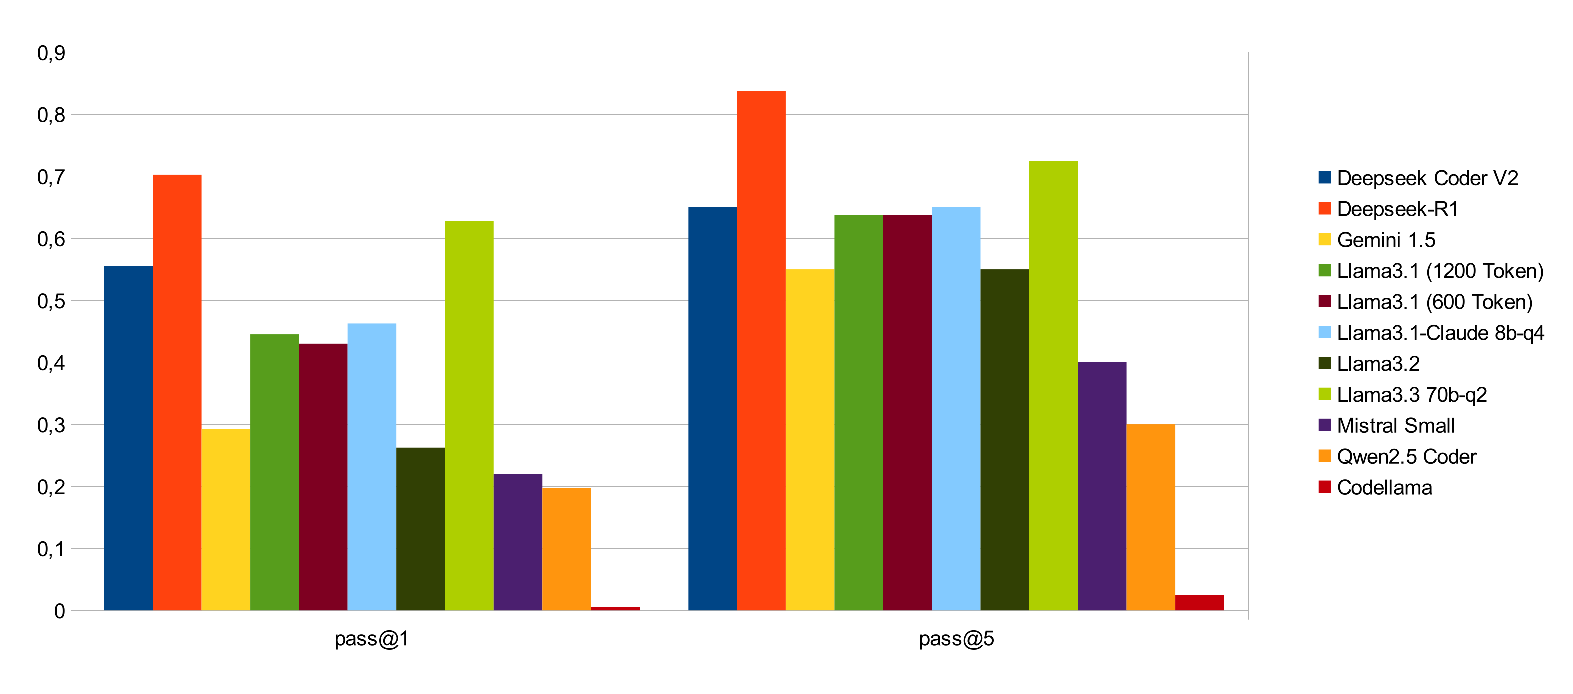
\includegraphics[width=\textwidth]{content/chapter_evaluation/images/llm_evaluation.eps}
	\centering
	\caption{Ergebnisse der pass@k-Methode für die Modelle}
	\label{img:pass_at_k_results_by_llm}
\end{figure}

Zwei weitere Modelle aus dem Open-Source-Bereich sind die Modelle \textit{Mistral-Small 22b} von der gleichnamigen Firma MistralAI und \textit{Qwen 2.5 Coder 32b}. Diese beiden Modelle schnitten im Vergleich nicht so gut ab. \vspace{0.2cm}

Das Modell \textit{Deepseek Coder V2 16b} welches an die Leistung von den Llama3.1 Modellen heranreicht.\vspace{0.2cm}
%Die Antworten von ChatGPT enthielten bei der ersten Abfrage Programmcode, alle weiteren Abfragen verwiesen auf den ersten Prompt. Eine Antwort ist in ?? dar gestellt, diese wurde in ähnlicher Weise immer wieder generiert.
%\hrulefill
%Der Code in deinem Kommentar ist identisch mit dem aktuellen Inhalt. Wenn du Än\-der\-ungen vornehmen möchtest, präzisiere bitte, was angepasst werden soll, und ich werde es umsetzen!
%\begin{flushright}
%	\textit{Generiert von ChatGPT 3.5}
%\end{flushright}
%\hrulefill

Ein weiteres Modell ist Gemini 15. von Google. Im Gegensatz zu den anderen Modellen, bringt Gemini nicht immer nur eine Lösung des Problems, sondern bietet weitere Ansätze, welche ebenfalls für das jeweilige Problem interessant sein könnten. Im folgenden Beispiel sind die verschiedenen Vorschläge des Modells in den Listings \ref{lst:gemini_result_php-3_1} bis \ref{lst:gemini_result_php-3_4} dargestellt, die beim PHP Problem 3 gefordert wurden. Die Aufgabenstellung in Kurzform war: \texttt{Gib den größten gemeinsamen Teiler von zwei ganzen Zahlen a und b zurück.}

\begin{lstlisting}[language=PHP,label=lst:gemini_result_php-3_1,caption={Gemini Ergebnis für das PHP-3 Problem Version 1}]
function greatestCommonDivisorRecursive($a, $b) {
  if ($b === 0) {
    return $a;
  } else {
    return greatestCommonDivisorRecursive($b, $a % $b);
  }
}
\end{lstlisting}

Neben den geforderten Lösung gab Gemini noch weitere Lösungsvorschläge aus. Das Listing \ref{lst:gemini_result_php-3_2} zeigt einen zweiten Lösungsansatz.\vspace{0.2cm}

\begin{lstlisting}[
	language=PHP,
	label=lst:gemini_result_php-3_2,
	caption={Gemini Ergebnisse für das PHP-3 Problem Version 2}
]
function greatestCommonDivisorBinary($a, b) {
  if ($a == 0) return $b;
  if ($b == 0) return $a;

  // Ensure a is odd
  if ($a % 2 == 0 && $b % 2 == 0)
    return 2 * greatestCommonDivisorBinary($a / 2, $b / 2);
  if ($a % 2 == 0) return greatestCommonDivisorBinary($a / 2, $b);
  if ($b % 2 == 0) return greatestCommonDivisorBinary($a, $b / 2);

  // a and b are odd
  if ($a > $b) return greatestCommonDivisorBinary($a - $b, b);
  return greatestCommonDivisorBinary($b - a, a);
}
\end{lstlisting}

Zu diesem Beispiel hat Gemini 1.5 noch weitere Lösungsansätze generiert. Diese sind in \ref{lst:gemini_result_php-3_3} und \ref{lst:gemini_result_php-3_4} zu sehen.

\begin{lstlisting}[
	language=PHP,
	label=lst:gemini_result_php-3_3,
	caption={Gemini Ergebnisse für das PHP-3 Problem Version 3}
]
function leastCommonMultiple(int $a, int $b): int {
  // kgV(a, b) = (a * b) / ggT(a, b)
  return abs($a * $b) / greatestCommonDivisor($a, $b);
}
\end{lstlisting}

\begin{lstlisting}[
	language=PHP,
	label=lst:gemini_result_php-3_4,
	caption={Gemini Ergebnisse für das PHP-3 Problem Version 4}
]
function greatestCommonDivisorMultiple(int ...$numbers): int {
  // ggT von mehreren Zahlen
  return array_reduce($numbers, 'greatestCommonDivisor');
}
\end{lstlisting}

Einige Aufgaben wurden von Gemini aber wie ein Chat behandelt. So hat das Modell Antworten generiert, die einer Konversation mit einem Chatbot ähneln, so wurde beispielsweise der folgende Text generiert, der einen Bezug zur zuvor gegebenen Antwort des Modells herstellt.

\hrulefill

\texttt{function greatestCommonDivisorRecursive(\$a, \$b) \{}

\texttt{\hspace{0.6cm} // ... (Rest der Funktion bleibt ähnlich)}

\texttt{\}}

\hrulefill

\begin{flushright}
	\textit{Generiert von Gemini 1.5}
\end{flushright}

Diese generierten Codeausschnitte haben die Tests nicht bestanden und wirken sich somit negativ auf die Auswertung aus.

\subsection{Nachteile der Evaluierung}
Es wird geprüft, ob der Code ohne Fehler ausführbar ist und die richtigen Ergebnisse liefert. Was dieser Test nicht evaluiert sind unter anderem vorhandene Codeerklärungen, Doc-Strings oder Code-Smells werden bei diesem Test nicht beachtet. Ebenso wird auch nicht der Codestandard geprüft.\vspace{0.2cm}

Benchmark prüfen, ob die Tests evtl. Fehler enthalten. Dies könnte sich beispielsweise in folgenden Probleme darstellen,

\begin{itemize}
	\item Tests sind falsch formuliert und die Abdeckung der geforderten Aufgabe wird nicht erfüllt, wodurch fehlerhafter generierter Code als korrekt bewertet wird.
	\item Fehler in den Musterlösungen können dazu führen, dass korrekte Lösungen als nicht bestanden gewertet werden.
	\item Mehrdeutige Aufgabenstellungen können ebenfalls das Ergebnis der Modelle negativ beeinflussen.
	\item Die Benchmark existieren bereit mehrere Jahre, sodass nicht ausgeschlossen werden kann, das Modelle explizit mit diesen Benchmarks trainiert wurden.
\end{itemize}

%--- Optimierung --------------------------------------------------------------------------------


\section{Optimierung der Ergebnisse}
Als Ziel der Optimierung gilt das die LLMs effizienten, präzisen und korrekten Code zu generieren. Ein Ansatz dies zu erreichen ist die Prompts zur Codegenerierung mithilfe einer LLMs zu erstellen oder zu verbessern.


% https://ki-techlab.de/ki-news/evaluierung-grosser-sprachmodelle-ein-technischer-leitfaden/

%\begin{tcolorbox}[
%	enhanced,
%	colback=BhtColorYellow!5!white,
%	colframe=BhtColorYellow!75!black,
%	title= HTML Startseite
%	]
%	Text in der Box
%\end{tcolorbox}

%\begin{tcolorbox}[
%	enhanced,
%	colback=BhtGrey!5!white,
%	colframe=BhtGrey!75!black!50,
%	title= ChatGPT 3.5
%	]
% Text in der Box
%\end{tcolorbox}


\chapter{Anwendungsszenarien}\label{chap:application_scenarios}

\chapter{Diskussion und Ausblick}\label{chap:discussion}
%Dieses Kapitel stellt eine Zusammenfassung der wichtigsten Ergebnisse dieser Arbeit auf, die zur Beantwortung der Thesen führen. Es werden zusammenfassend die Grenzen und Einschränkungen geklärt, zu denen die Evaluation durchgeführt wurde. Des Weiteren werden Impulse für weitere Forschungen diskutiert. Das Kapitel endet mit einer praktischen Anwendung, bei der die Ergebnisse dieser Arbeit angewandt werden können.

%Vergleich Stand der Forschung: fehlt noch, muss in Thesen einfließen

\section{Bewertung der Zielsetzung und Thesen}
% 3. These: Optimierung ohne Modellanpassung, nur Prompt Engineering
Die Erkenntnisse aus den Experimenten dieser Arbeit bestätigen die aufgestellte dritte These (T3) aus Kapitel \ref{sec:goals_of_the_work}. Eine Optimierung der Eingabeaufforderungen für die Webanwendungsentwicklung lässt sich ohne Änderung der Modellparameter erreichen und bewirken eine signifikante Verbesserung der Ergebnisse. Die Modelle wurden bereits mit Programmiersprachen, die für Webanwendungsentwicklung essenziell sind, wie beispielsweise PHP, trainiert und diese Daten, in Form von Programmcode sind in den Modellen abrufbar. Entscheidend hierbei ist die Art und Weise wie die Gestaltung der Eingabeaufforderungen umgesetzt wird. Diese Optimierung erfolgt durch das \texttt{DSPy} Framework für die meisten Modelle automatisch.\vspace{0.2cm}

% Hat nicht funktioniert.
Dennoch hat das \texttt{DSPy} Framework, auf einige Modelle eine negative Auswirkung. Der generierte Code schnitt in der Evaluation mit den HumanEval-XL Proben schlechter ab. Der Grund konnte zurzeit nicht geklärt werden. Eine Annahme ist, dass der deklarative Ansatz von DSPy mit den komplexeren Datenstrukturen und Modulketten die LLMs zu inkonsistenten Antworten leitet. In diesen Fällen sollte weitere Frameworks, wie beispielsweise \textit{AdalFlow} oder \textit{LamaIndex} für die Optimierung in Betracht gezogen werden.\vspace{0.2cm}

% Es gibt Fehler bei der Verwendung von DSPy.
Die Tests haben weiterhin gezeigt, dass einige Modelle nicht mit dem \texttt{DSPy} Framework zusammenarbeiten. Auch hier konnte nicht abschließend geklärt werden, ob die Fehlerquelle bei der eingesetzten Hardware zu suchen ist oder ob das Framework selbst Probleme mit den Antworten dieser Modelle hat. Bei Modellen, die dieses Verhalten zeigen, sollte geprüft werden, ob auch hier die Wahl auf ein anderes Framework fallen kann.\vspace{0.2cm}

Gerade mit der Arbeit von Closed-Source-Modellen, bei der die Modelle gar nicht oder nur sehr bedingt angepasst werden können, sind die Optimierungen der Eingabeaufforderungen essenziell.\vspace{0.2cm}

% 2. These: Benckmarks sind ungeeignet
Alle Evaluierungen wurden mit den HumanEval-XL durchgeführt. Mit den gewonnenen Erkenntnissen aus dieser Arbeit lässt sich die zweite These (T2) nur bedingt bestätigen. Ein einzelner Benchmark hat nicht ausreichend Aussagekraft, um eine LLM hinreichend zu bewerten. Diese Benchmarks eignen sich um einen ersten Eindruck von den Modellen zu erhalten. Hierbei können erste Eindrücke über deren Stärken und Schwächen gesammelt werden. Wie auch in \cite{zhang-2024} wird die Auffassung vertreten, dass diese Probe grundlegende Codeproblematiken testen, die nicht mit den realen Anforderungen von Entwicklern übereinstimmen. In dem Onlineartikel \cite{albrecht-2023} heißt es \glqq \textit{...liefert Code, der zwar nicht immer direkt nutzbar ist, nach einer Überarbeitung aber schon recht überzeugend läuft.}\grqq. Diese Aussagen deuten darauf hin, dass Programmierer andere Anforderungen an LLMs stellen, die zurzeit mit Benchmarks nur in engen Grenzen abgedeckt werden können.
Die menschliche Intelligenz ist in der Lage aus generiertem Code und eigenem Wissen, die Programmteile herauszufiltern welche zur Lösung eines Problems beitragen. Entwickler stellen meist sehr komplexe Anforderungen, um die ihnen gestellten Probleme zu lösen. Diese Komplexität wird durch die Benchmarks nicht abgedeckt.\vspace{0.2cm}

% 1. These: LLMs effizientere Webanwendungsentwicklung. Wichtig ist die Evaluierung
In den letzten Jahren hat generative KI auch die Arbeit der Entwickler stark beeinflusst. So ist in \cite{focus-online-2025} die Rede von einem Programmierer, der seine Aufgabe abbrach, Zitat: \glqq \textit{weil er keinen Zugang zu seinem virtuellen Assistenten hatte. ''Ich kann einfach nicht mehr ohne die Hilfe der KI programmieren''}\grqq \ so der Entwickler. In \cite{company_gartner_2024}, einem Artikel von Gartner, wird behauptet das bis zum Jahr 2027, 80\% der Ingenieure eine Weiterbildung für generative KI benötigen. Dies hebt ebenfalls den Trend der nächsten Jahre hervor, das generative KI die Softwareentwicklung maßgeblich beeinflussen wird.
% Zu den Modellen.
Die Beliebtheit von KI Anwendungen wächst bei Softwareentwicklern immer weiter und dies gilt auch für den Bereich der Webanwendungsentwicklung. Dabei nutzen viele Entwickler, KI Modellen von US amerikanischen Unternehmen wie Athropic, Google oder OpenAI die bereits sehr gut entwickelte Chatbots und APIs anbieten, welche für die Integration in Tools zur Codegenerierung eingesetzt werden können. Zurzeit hat Mistral, eine europäische KI-Entwicklungsfirma einen neuen Chatbot, mit names \textit{Le Chat} herausgebracht, der Kokurrenz zu den amerikanischen Konzernen gesehen wird. Die KI-Entwicklungsfirma \textit{Deepseek} aus China hat ein Modell entwickelt, das wie Mistral in Konkurrenz zu den amerikanischen Modellen steht. Neben diese kommerziellen Closed-Source-Modelle gibt es eine Reihe von Open-Source-Modellen, welche ebenfalls hervorragende Resultate für die Generierung von Code zeigen, wie die Ergebnisse dieser Arbeit beweisen. Um so wichtiger ist es die Stärken und Schwächen der Modelle zu kennen und welche Methoden, zur effektiven Nutzung von Eingabeaufforderungen einzusetzen sind. Mit diesen Kenntnissen wird die, in der Arbeit aufgestellte dritte These (T3) bewiesen. Ki kann und wird die Webanwendungsentwicklung maßgeblich beeinflussen.\vspace{0.2cm}

Gerade die einfache und effiziente Suche mithilfe der LLMs bring einen zeitlichen Vorteil, dessen Ergebnisse bereits mit einfachen Tests überprüft werden können. LLMs reduzieren die Suche nach geeigneten Frameworks und Technologien und liefern fast immer funktionsfähigen Code. Dies gilt für die Integration in \acrshort{IDE} wie auch die Nutzung eines Chatbots.

\section{Grenzen und Einschränkungen}
%Kleine Beteiligung der Closed-Source-Modelle aufgrund der Kosten.
Die in dieser Arbeit evaluierten und optimierten Modelle, waren hauptsächlich Open-Source-Modelle. Alle diese Modelle wurden von der Plattform Ollama bereitgestellt. Zwei Ausnahmen gab es bei der Evaluierung, hierbei handelt es sich um \textit{Gemini 1.5} von Google und \textit{ChatGPT 4} von OpenAI.\vspace{0.2cm}

%Benchmark nur den HumanEval-XL, mit 80 Proben.
Für die Evaluierung der Modelle ist nur der \textit{HumanEval-XL} angewandt worden. Die meisten Benchmarks prüfen LLMs mit Python oder Java Proben. Eine Evaluierung mit spezifischen Sprachen für Webanwendungsentwicklung wie PHP, bieten nur wenige Benchmarks.\vspace{0.2cm}

%Nur langchain und DPSy
Die Auswahl der getesteten Frameworks, welche die Kommunikation zu den LLMs und somit zum Ollama-Server herstellten, waren begrenzt auf \texttt{langchain} und \texttt{DSPy}.\vspace{0.2cm}

\section{Impulse für zukünftige Forschungen}
%Ein interessantes Feld für die Forschung ist die Nutzung generativer KI und welche Auswirkungen dies auf das menschliche Denken und Handeln hat. In der Studie \cite{chiriatti-2024} wird von einem System 0 gesprochen, welches neben den bekannten 
%\begin{enumerate}
%	\item System 1: schnelles,intuitives und automatisches Denken
%	\item System 2: langsameres, analytisches und reflektierteres Denken
%\end{enumerate}

%eingeführt wird. Hierbei handelt es sich um ein Denken, welches die KI für den Menschen übernimmt. Entscheidungen und Daten werden durch die KI übernommen. Ein externes System, ähnlich wie eine USB-Festplatte eines PCs.\vspace{0.2cm}
% Immer neue Modelle
Die KI-Entwicklungsfirmen bringen immer neue Modelle auf dem Markt, die schon mit einer sehr kleinen Anzahl vom Parametern gute Ergebnisse liefern. Hier könnte eine Studie zeigen, ob \textit{Small Language Models} (SLM) mit den \textit{Large Language Models} (LLM), im Bereich der Webanwendungsentwicklung konkurrieren können. Ein Beispiel für ein SML ist das Modelle \textit{Phi} von Mirosoft, welches beispielsweise unter \cite{phi2_huggingface_2024} heruntergeladen werden kann. Wird ein Modell für die Codegenerierung eingesetzt und dahin gehend optimiert, ist die Menge an Parametern nicht erforderlich. Es existieren bereits einige Studien zu diesem Thema. Beispielsweise wird in \cite{hu-2024} eine allgemeine Verbesserung des Benutzererlebnisses untersucht und in \cite{irugalbandara-2023} wird eine Reduzierung der Kosten in Produktionsumgebungen vorgestellt.\vspace{0.2cm}
%Inwieweit können auch \textit{Small Language Models} für Programmieraufgaben eingesetzt werden. Könnte der enorme Energiebedarf und Ressourcen der LLMs durch SLMs ersetzt werden? Siehe \href{https://medium.com/@nageshmashette32/small-language-models-slms-305597c9edf2}{Small Language Models (SLMs)} oder \href{https://medium.com/version-1/small-but-powerful-a-deep-dive-into-small-language-models-slms-b793bdb002f2}{Small but Powerful: A Deep Dive into Small Language Models (SLMs)}. Eine weitere Forschung kann die Evaluation sein, ob Finetuned SLMs, wie Phi-2, Google Gemini Nano oder Metas Llama-2-13b bessere Ergebnisse liefern, als die LLMs.\vspace{0.2cm}

% Andere Benchmakrs eigene entwickeln.
Des Weiteren sollte Unternehmen oder Entwickler weitere Benchmarks in Betracht ziehen und die Brauchbarkeit von LLMs für die Webanwendungsentwicklung evaluieren. Interessant wäre die Prüfung, ob die Verwendung mehrerer Benchmarks zu einer besseren Bewertung der LLMs führt.\vspace{0.2cm}

Da die meisten Benchmarks auf statische Analysen ausgelegt sind und die LLMs nur bedingtes oder klein deterministisches Verhalten zeigen, kann eine weitere Forschung dahin gehen, einen Benchmark zu erstellen, der auf die dynamischen Antworten der LLMs besser eingehen könnte. Speziell für die PHP-Entwicklung wäre eine Untersuchung interessant, bei der die Evaluierung mit externer Tool wie \textit{SonarQube}, \textit{PHPBench}, \textit{PHPUnit} oder \textit{PHPMetrics} durchgeführt und dadurch eine verbesserte Bewertung der LLMs  erreicht wird.  Analog kann so ein Benchmark auf für andere relevante Programmiersprachen der Webentwicklung, wie beispielsweise JavaScript, Java und Ruby ausgeweitet werden.\vspace{0.2cm}

% Einführung in Firmen und Schluung der Mitarbeiter.
Ein weiteres mögliches Themenfeld ist die Einführung einer KI gestützten Softwareentwicklung für Webanwendungen mit Firmenrichtlinien. Der Fokus sollte hierbei auf das Auswahlverfahren der Modelle liegen mit Blick auf die möglichen Benchmarks und dem Evaluierungsverfahren. Wie lassen sich Entwickler frühzeitig in die Auswahl der Modelle einbeziehen und welche Möglichkeiten bestehen für Entwickler schon während dieses Prozesses ihre Kenntnisse im Bereich von generativer KI zu erweitern oder vertiefen, sodass effektives Entwickeln von Anfang an erfolgen kann.\vspace{0.2cm}
%\begin{tcolorbox}[
%	enhanced,
%	breakable,
%	colback=red!5!white,
%	colframe=red!75!black!50,
%	title= Mein roter Faden: noch was zum Testen
%	]
%	Ein Tool zur Orchestrierung von Multi-Agenten-Systemen \href{https://community.openai.com/t/introducing-swarm-js-node-js-implementation-of-openai-swarm/977510}{OpenAI Swarm}, gefunden auf \href{https://karrierewelt.golem.de/blogs/karriere-ratgeber/bot-belegschaft-mit-entlastungspotenzial-ki-agenten-fur-den-arbeitsalltag-in-der-testphase-1}{Golem | Karrierrewelt}.
%\end{tcolorbox}

\section{Praktische Anwendung}
%Praktische Anwendung: Eine Diskussion der möglichen Anwendungen der Ergebnisse. In welchen Unternehmen und welche realen Anwendungen können die Ergebnisse eingesetzt werden.
% Konkreter Fall
In der kommenden Zeit wird die Entwicklung der LLM weiter voranschreiten, dies wird zu weiteren Verbesserungen bei den Ausgaben der LLMs führen. Dennoch sollte der Focus auf eine einheitliche Vorgehensweise liegen. Somit werden nicht nur gleiche Standards beim Code geschaffen, zudem wird ein einheitliches Know-How der Mitarbeiter realisiert. Dies wird langfristig dazu führen, dass die Entwicklung von Webanwendungen mithilfe generativer KI, die Arbeit der Entwickler effizienter gestaltet und sich somit auf die Kosten und Ressourcen der Unternehmen auswirkt.\vspace{0.2cm}

% Nutzen/Vorteil
Die Auswahl der Anbieter wird, durch deren ständig wachsender Anzahl immer schwieriger. Die in dieser Arbeit evaluierten Modelle, können Unternehmen nutzen, um einen Einstieg in das Thema zubekommen und schlägt Modelle vor, welche sich für die Generierung von Programmcode in der Webanwendungsentwicklung eigenen. Des Weiteren unterstützt diese Arbeit sie den bei ersten Versuchen, weitere neue LLMs zu evaluieren und das optimale Modell für ihre Prozesse zu finden. Die Mehrheit der Entwickler und Unternehmen nutzt zurzeit kommerzielle Modelle großer Anbieter, da die Nutzung der Chatbots und schnelle, unkomplizierte Verwendung der APIs mit wenig Aufwand realisierbar ist. Durch das zunehmende breite Interesse an generativer KI, wurden Möglichkeiten geschaffen Open-Source-Modelle in der eigenen Infrastruktur einzubinden und diese zu verwenden. Dies kann, wie schon zuvor besprochen zur Senkung der Kosten beitragen. Besonders die Abrechnung der Tokens ist ein interessanter Punkt, der nicht immer eindeutig nachvollziehbar ist. Der Kostenaspekt zwischen \textit{Open-Source} und \textit{Closed-Source} Modellen, wurde schon aufgegriffen, diskutiert und bringt laut \cite{irugalbandara-2023} eine große Ersparnis, was nicht nur für kleine und mittlere Unternehmen interessant werden kann. Wie in dieser Arbeit gezeigt, liefern die Open-Source-Modelle hervorragende Ergebnisse für die Aufgaben in der Webanwendungsentwicklung, oft bessere als die kommerziellen Closed-Source-Modelle.\vspace{0.2cm}

% Implementierung
Unabhängig von der Auswahl des Modells sollten Unternehmen für die Entwickler einheitliche Schnittstellen zu den Modellen bereitstellen. Zum Einem können die Eingabeaufforderungen, wie in dieser Arbeit beschrieben, mittels verschiedener Frameworks oder anderer Methoden angepasst werden. Zum anderen können die abgesetzten Prompts verwendet finden, um Modelle weiter, durch \glqq Fine-Tuning\grqq \ zu optimieren. Eine weitere Möglichkeit besteht darin die Prompts auszuwerten und den Wissensstand der Entwickler zu prüfen und ggf. mit gezielten Schulungsmaßnahmen das Entwicklungsteam zu fördern.\vspace{0.2cm}

Ein weiterer Vorteil dieser Methode ist, dass die Prompts mit verschiedenen Metadaten angereichert und Ansätze wie \textit{Personas}, \textit{Beispielen} und \textit{zusätzlichem Kontext} umgesetzt werden können. Vorstellbar wäre auch die Integration eines RAG, welches auf Daten der eigenen Entwickler und bereits umgesetzter Softwarelösungen zurückgreifen kann.\vspace{0.2cm}

% Example
Die Abbildung \ref{img:example_firm_integration} zeigt das zuvor beschriebene Beispiel für die Integration einer LLM in den Prozess zur Programmcodegenerierung. Die Entwickler stellen ihre Eingabeaufforderungen an den Agenten. Das erfolgt über ein Eingabeformular oder als Plug-in einer IDE. Über das Plug-in wird der generierte Code direkt in den aktuellen Programmcode übernommen, das Formular bietet die Möglichkeit weitere Fragen an die LLM, welche nicht im Code erscheinen sollen. Dies könnten allgemeine Fragen zur Architektur oder Fragen zur Beurteilung von Tools beinhalten. So werden alle Fragen und Probleme erfasst, vor die Entwickler stehen.
% Der Agent
In einem ersten Schritt könnte der Agent als verwendetes Framework implementiert und später durch einen echten Agenten ersetzt werden. Der Agent leitet den optimierten Prompt an die LLM, wertet die Antwort aus und sendet das Ergebnis an den Entwickler zurück. Zusätzlich werden die Prompts aufgezeichnet und in einer Datenbank gespeichert. In der Abbildung wird die Datenbank als \texttt{Logs} bezeichnet. Für die grün dargestellten Elemente, in der Abbildung \ref{img:example_firm_integration} sind in dieser Arbeit bereits Ansätze und Lösungsvorschläge vorgestellt und besprochen wurden.\vspace{0.2cm}

\begin{figure}[!ht]
	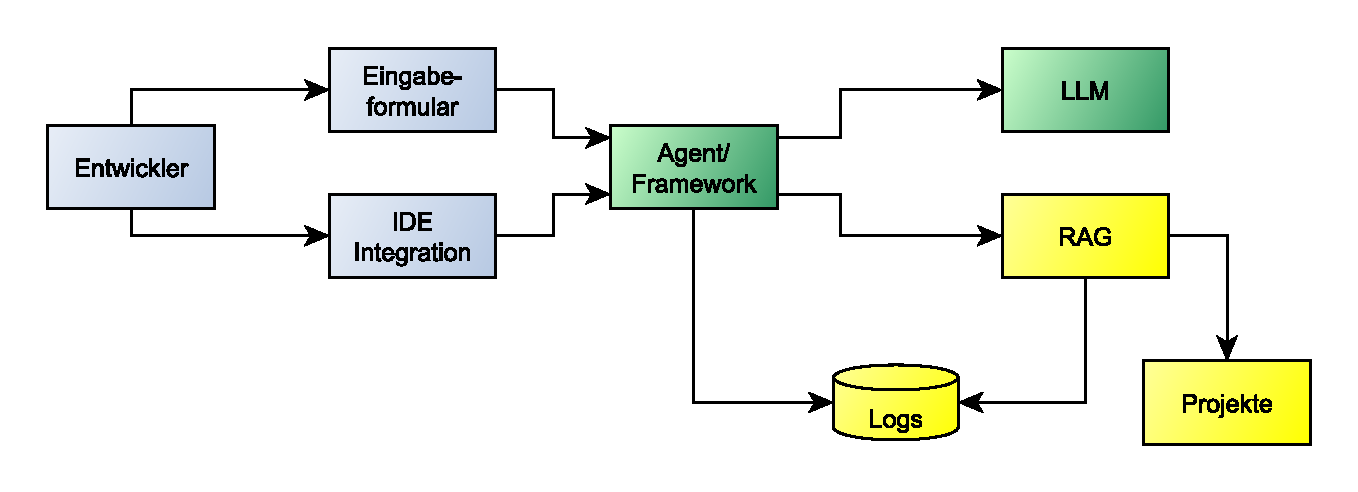
\includegraphics[width=0.9\textwidth]{content/chapter_discussion/images/anwendungsbeispiel.eps}
	\centering
	\caption{Anwendungsbeispiel für die Integration einer LLM}
	\label{img:example_firm_integration}
\end{figure}

Eine mögliche Erweiterung ist das Austauschen des Frameworks und der Einsatz eines Agenten. Im Weiteren kann ein \textit{Retrieval Augmented Generation} (\acrshort{RAG}) implementiert werden, um auf vorhandene firmenintern Daten zuzugreifen. Diese Daten können bereits gestellte Prompts der Entwickler oder vorhandener Code aus fertigen Projekten sein. Mit dem, in dieser Arbeit vorgestellten \texttt{DSPy} Framework können Agenten und RAG implementiert werden.\vspace{0.2cm}

Abschließend wird in Abbildung \ref{img:example_chat_form} ein Beispiel für ein einfaches Chat-Formular gezeigt. Weitere Formularfelder können im Formular hinzugefügt und der LLM als zusätzliche Metadaten oder Anweisungen mitgeteilt werden.\vspace{0.2cm}

\begin{figure}[!ht]
	
\includegraphics[width=0.8\textwidth]{content/chapter_discussion/images/chatbot_form_example.eps}
	\centering
	\caption{Anwendungsbeispiel für ein Eingabeformular für Prompts}
	\label{img:example_chat_form}
\end{figure}

%Blaupause für Prompting \href{https://piamedia.com/wp-content/uploads/2024/09/PIAM_Whitepaper_LLM-Halluzinationen_DE.pdf}{Das Geheimnis hinter LLM-Halluzinationen} [S. 16 ff.] noch testen und evaluieren.

%\href{https://arxiv.org/html/2501.16998v1}{Große Sprachmodelle zur Codegenerierung: Die Perspektive der Praktiker}

%Zur Optimierung des generierten Codes kann auch die freie Wahl der Softwarekomponenten durch die LLMs betragen. Wie in \cite{chen-2021} beschrieben können Nutzer, anstatt in Suchmaschinen beispielsweise die Vorteilen und Nachteile von \texttt{PyTorch} und \texttt{Tensorflow} zu vergleichen, kann das die LLM übernehmen und als Prompt wird nur \texttt{\# import machine learning package} angegeben.\vspace{0.2cm}

%Wie in [Quelle ist weg] beschrieben nimmt das Lesen von Programm zehn mal mehr Zeit in Anspruch, als Code zu schreiben. Diese Arbeit kann ebenfalls durch eine LLM übernommen werden.


\chapter{Fazit}\label{chap:conclusion}

% Documents
% https://arxiv.org/abs/2109.04738: On the validity of pre-trained transformers for natural language processing in the software engineering domain
% https://arxiv.org/abs/2204.03214: Transformer-Based Language Models for Software Vulnerability Detection
%
% Tutorials
% https://towardsdatascience.com/building-a-python-code-generator-4b476eec5804